\documentclass[a4paper,landscape]{article}
\usepackage[margin=1in]{geometry}
\usepackage[operators]{cryptocode}
\usepackage{tikz}
\renewcommand\O[1]{\ensuremath{\mathsf{#1}}}
\newcommand{\M}[1]{\ensuremath{\text{\texttt{#1}}}}
\newcommand{\n}[1]{\ensuremath{\mathit{#1}}}
\tikzstyle{package} = [inner sep=1pt,align=center,rounded corners,draw,minimum width=2cm,minimum height=1cm,font=\small]
\tikzstyle{onarrow} = [inner sep=1pt,font=\scriptsize,anchor=east,at end,xshift=-0.1mm,align=left,fill=white]
\title{Modprfreal Game}
\begin{document}
\maketitle
\begin{center}
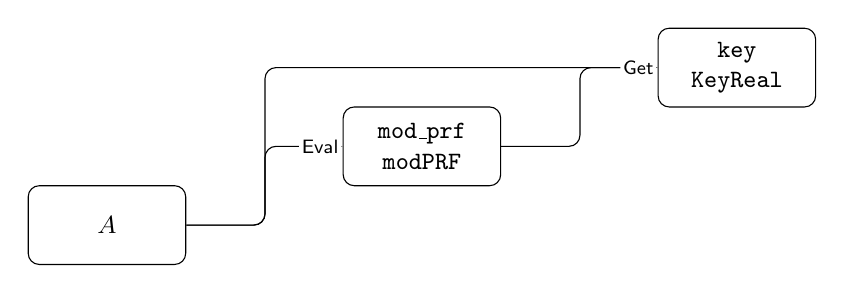
\begin{tikzpicture}
\node[align=center,package,fill=white] (node1) at (0, 0) {\M{key}\\\M{KeyReal}};
\node[align=center,package,fill=white] (node0) at (-4, -1) {\M{mod\_prf}\\\M{modPRF}};
\draw[-latex,rounded corners] (node0) -- ($(node0.east) + (1,0)$) |- node[onarrow] {\O{Set}} (node1);
\node[package] (nodea) at (-8, -2) {$A$};
\draw[-latex,rounded corners] (nodea) -- ($(nodea.east) + (1,0)$) |- node[onarrow] {\O{Eval}} (node0);
\draw[-latex,rounded corners] (nodea) -- ($(nodea.east) + (1,0)$) |- node[onarrow] {\O{Get}} (node1);
\end{tikzpicture}

\end{center}
\begin{center}
\begin{pcvstack}\underline{\underline{\M{mod\_prf}}}\\\begin{pchstack}
\procedure{\O{Eval}(h)}{
\pcif \n{ltk} = \O{none}(\O{Bits("n")}) \pcthen\\
\pcind\n{ltk\_} \stackrel{1}{\sample} \O{Bits("n")}\\
\pcind \n{ltk} \gets \O{some}(\n{ltk\_})\\
 \n{ltk\_} \gets \O{unwrap}(\n{ltk})\\
 \n{k} \gets \O{prf}(\n{ltk\_}, \n{h})\\
\n{\_} \stackrel{\mathsf{\tiny{invoke}}}{\gets} \O{Set}(\n{k}, \n{h}) \pccomment{Pkg: key}
}
\pchspace
\end{pchstack}\end{pcvstack}

\end{center}
\begin{center}
\begin{pcvstack}\underline{\underline{\M{key}}}\\\begin{pchstack}
\procedure{\O{Set}(k, h)}{
\pcif \n{K}[\n{h}] = \O{none}(\O{Bits("n")}) \pcthen\\
\pcind\n{k} \stackrel{2}{\sample} \O{Bits("n")}\\
\pcind \n{K}[\n{h}] \gets \O{some}(\n{k})\\
}
\pchspace
\procedure{\O{Get}(h)}{
 \pcreturn \O{unwrap}(\n{K}[\n{h}])\\
}
\pchspace
\end{pchstack}\end{pcvstack}

\end{center}
\end{document}
